\chapter{Results}

\section{Breadboard Testing}

The intial testing aimed to completely lay out the network configuration as the sending the sensor data was the relatively easy part. The USB connector attached to the breadboard would supply power to all of the devices with the native 5V and regulated 3V3 (using the LM1117-3V3 Regulator) supply voltages with a wall charging adapter or even a power bank which increased portability and made testing easier. Various networking libraries for the NRF24 were tested out. We also conducted range tests with varying transmission bit rates and signal strength and found that the NRF24 satisfied our requirements.

This was the foundation for our project as these results confirmed our concept and so we moved on to making the PCBs while simultaneously conducting further tests and code development on these breadboard prototypes. 

\section{Final Device}

\begin{center}
		
		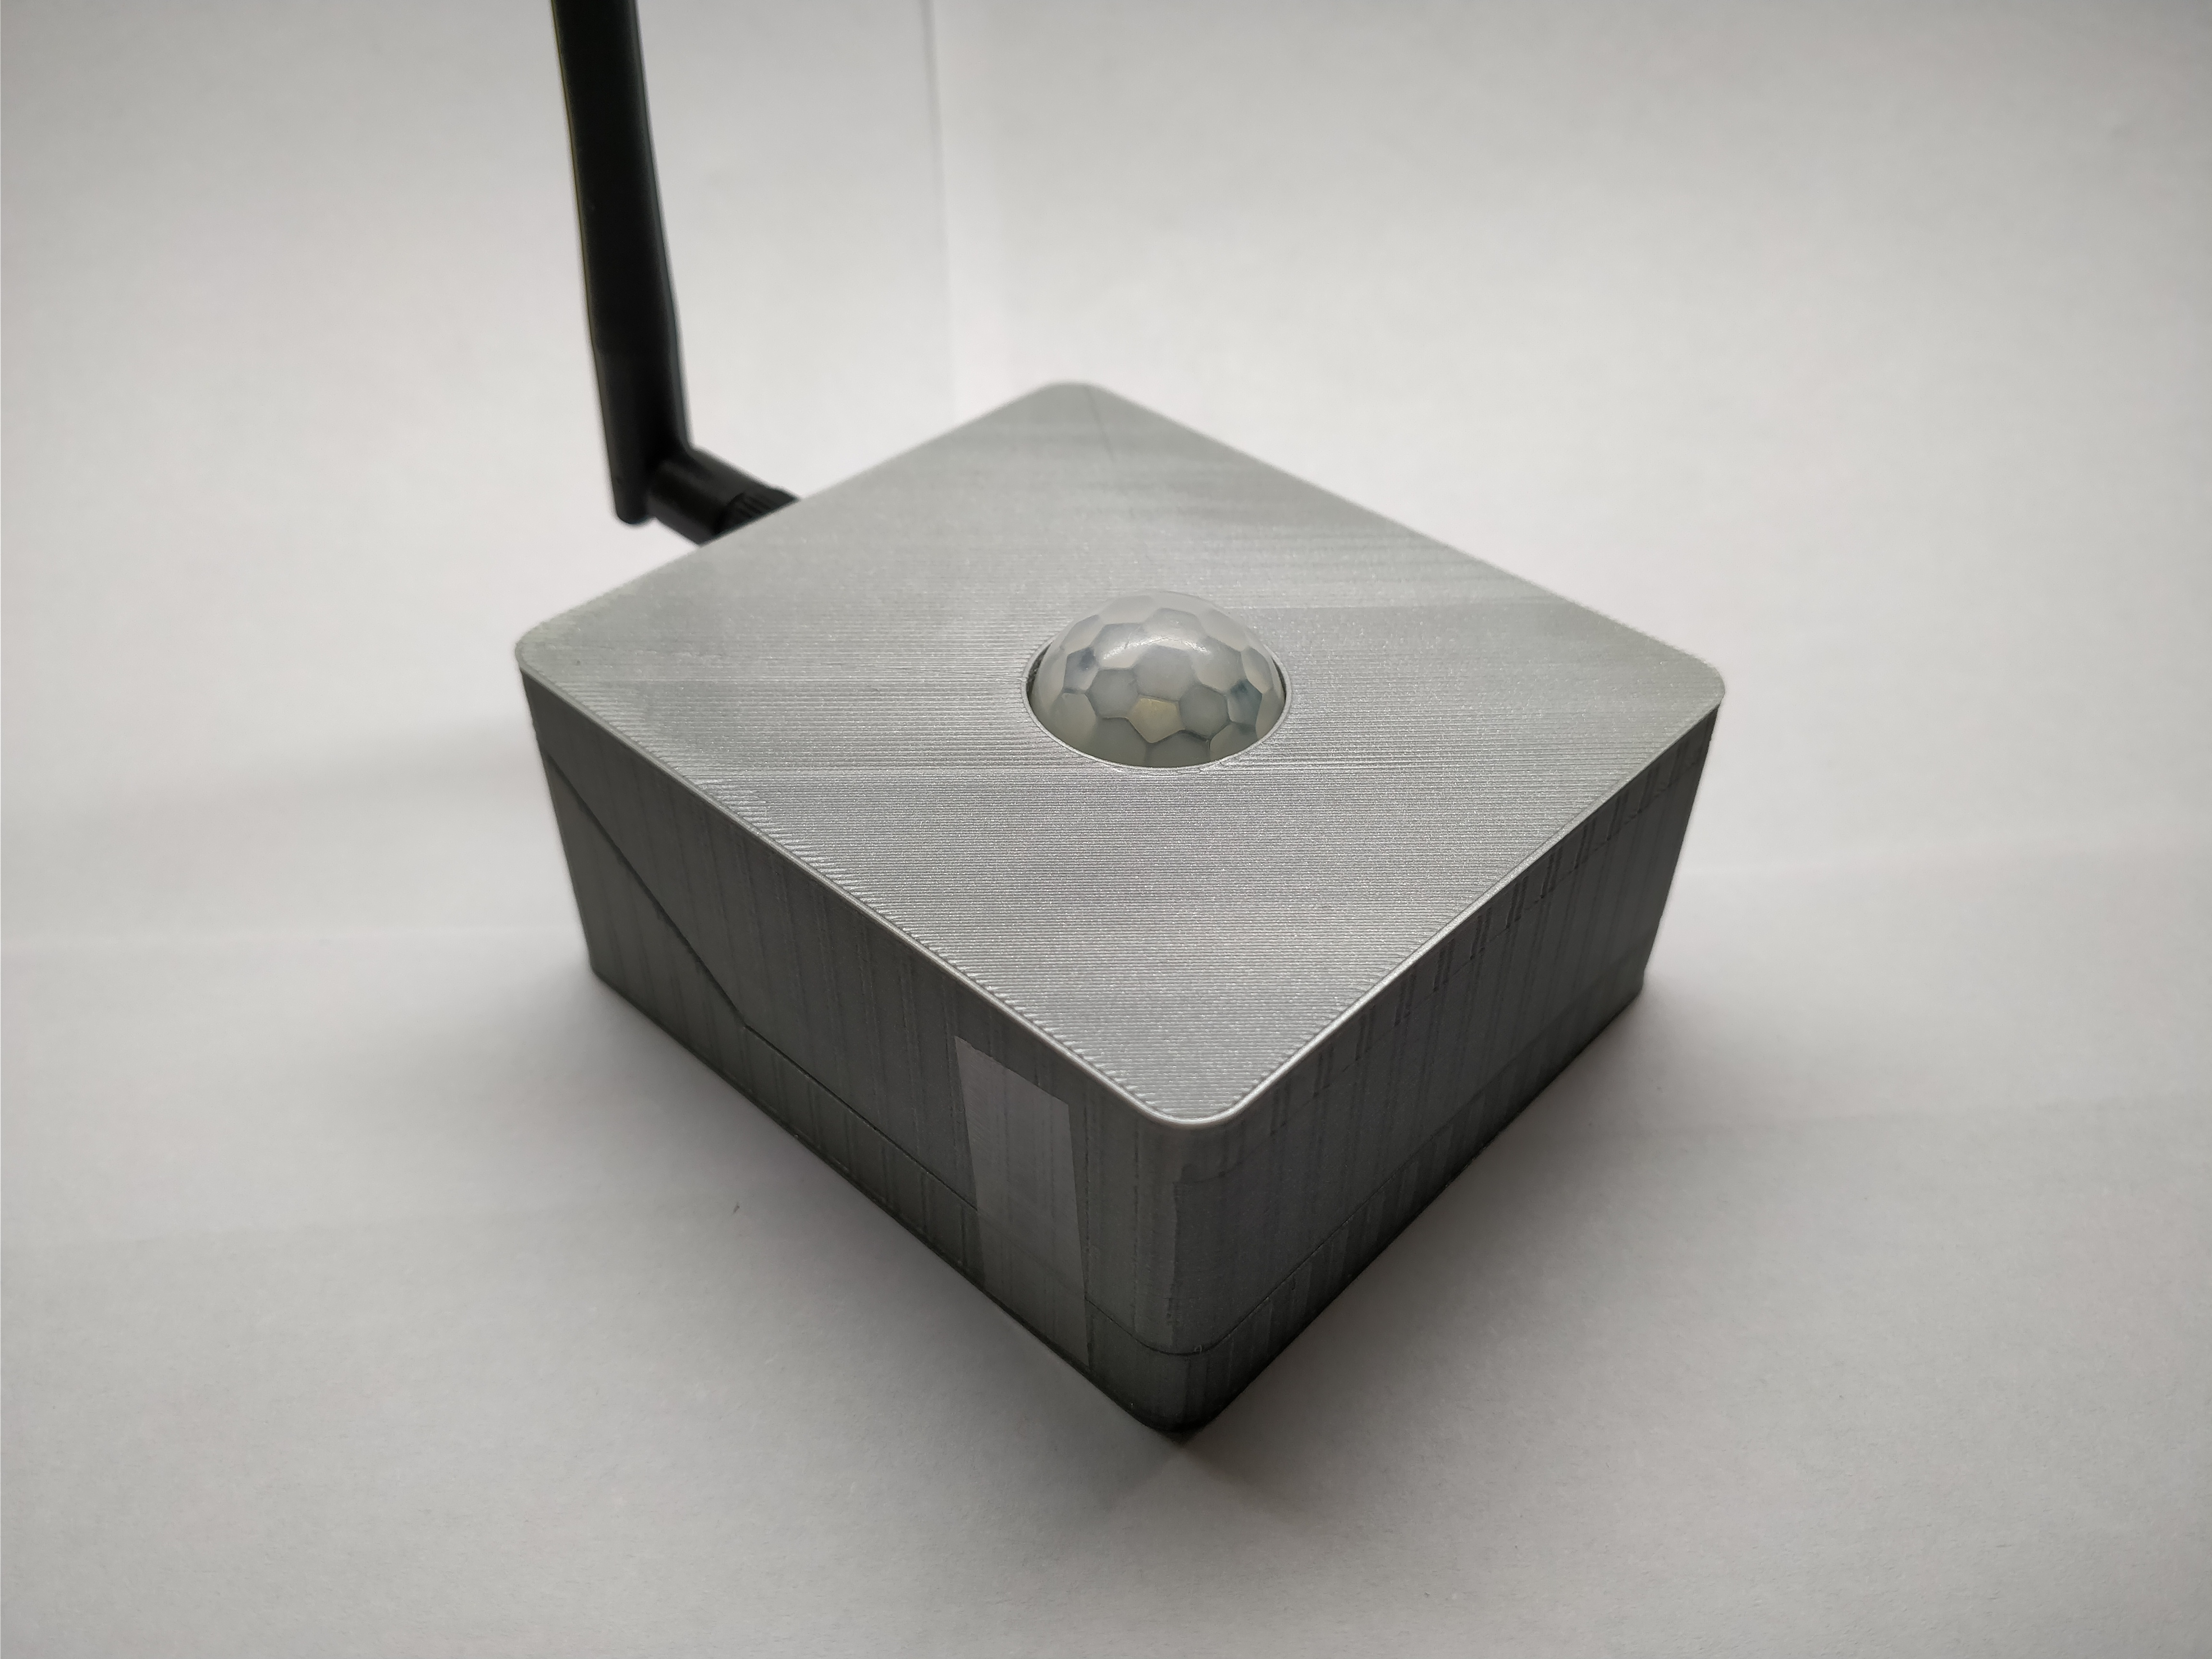
\includegraphics[scale=.07]{FinalProduct.jpg}
		
		Final Assembled Device

\end{center}


All the end nodes stay in a deep sleep state. They wake up only when a change of state in the PIR sensor is detected or when the WDT overflows. 

When motion is detected the device wakes up from its deep sleep state using interrupts and then transmits the required information and goes back to its deep sleep state. 
The devices also periodically wake up and send the state when the WDT overflows. This is so that if a device fails the master can sense that the device hasn't transmitted anything recently and then that device can be marked offline by the user.

The routers are always awake and listening so that they can route information between the devices and the master whenever required. They can be battery powered or can be powered using a mains adapter.

The current of the end nodes is 18mA when transmitting but it is only 80$\mu$A when it is in standby mode. This will significantly improve the battery life of the devices.

All the devices are configured in a tree network configuration to increase the range of the network. Each NRF24 Module can support upto 6 slave devices simultaneously, so the network has to be designed appropriately while setting it up in any real environment.

\vspace{10pt}
\begin{center}
	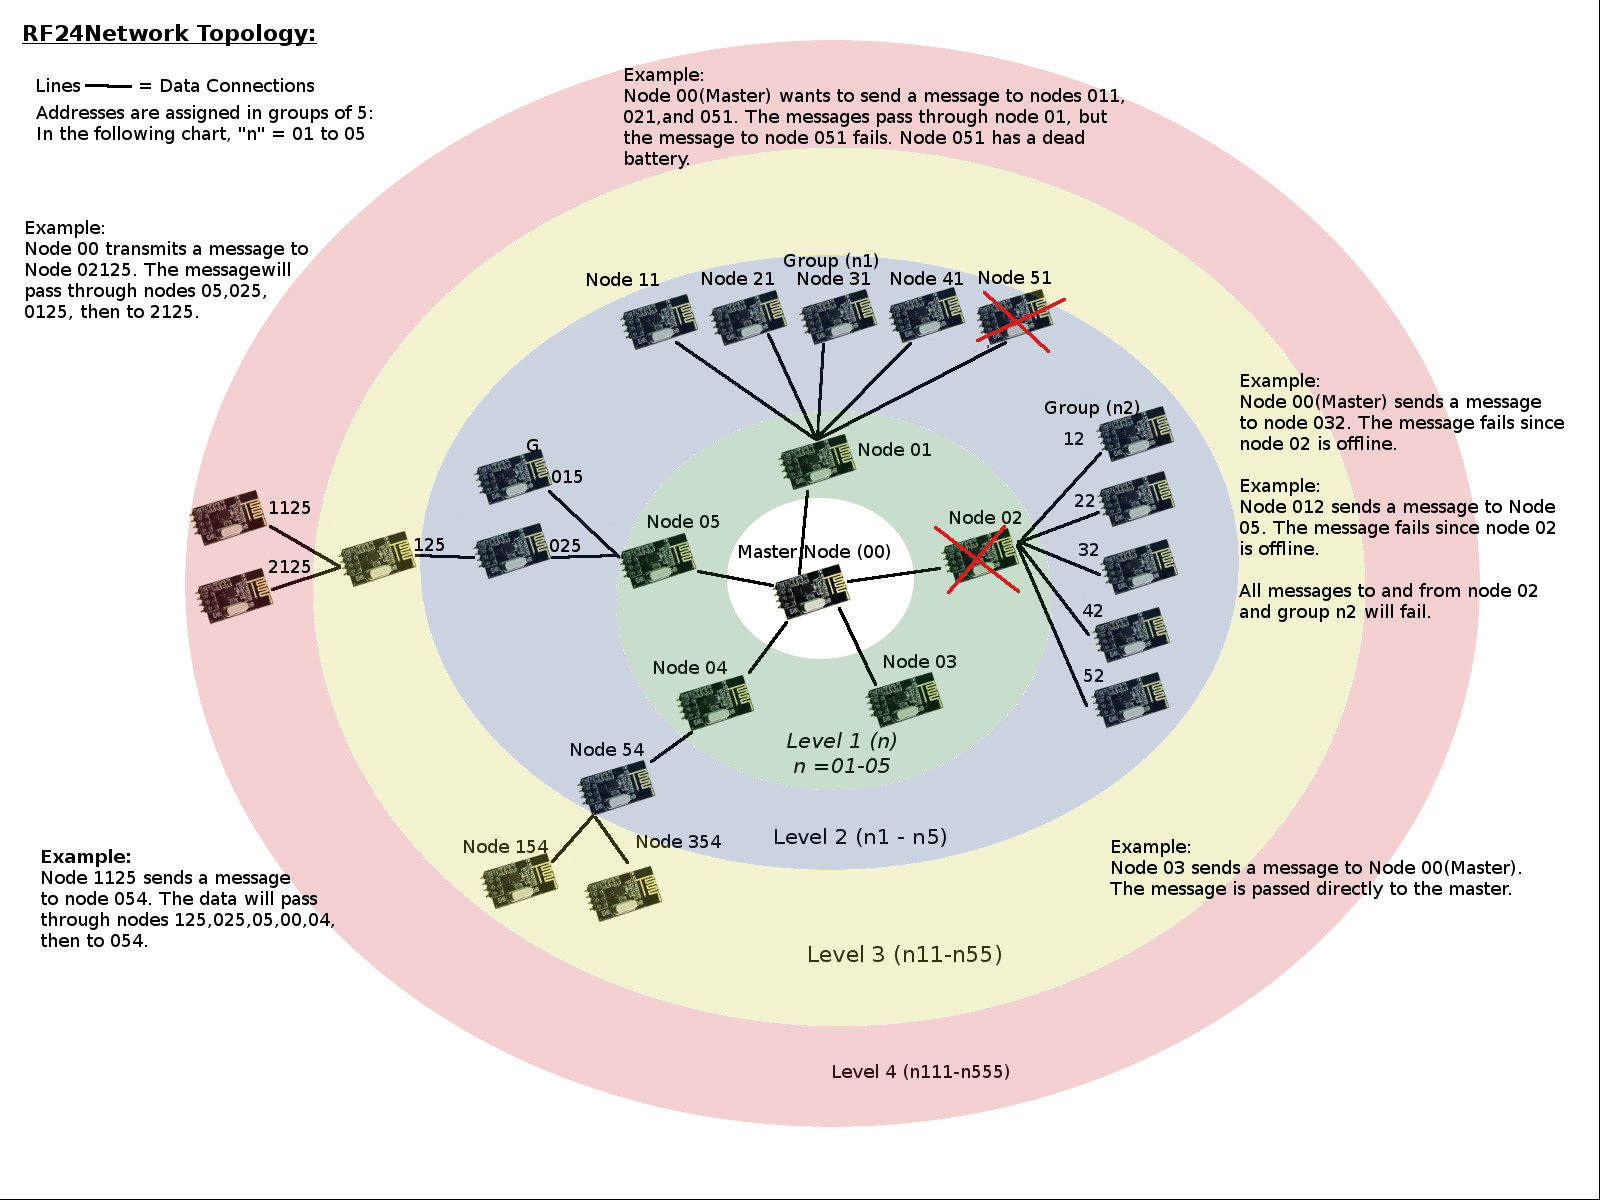
\includegraphics[scale=0.25]{TreeNW.jpg}
	
	Tree network topology
\end{center}

\pagebreak

\section{Cost per Device}

The final cost per device is about 900Rs. This is subject to change as per the source of the components. Also this is the cost of building the prototype. Large volume production cost will be much lower.
The cost distribution per device is as follows
\\
\begin{center}
	\begin{tabular}{|c|c|}
		\hline
		\textbf{Part} & \textbf{Cost}	\\			\hline
		NRF24l01+ radio transceiver module & 250 \\	\hline
		PCB & 120 \\								\hline
		ATmega328P-PU &120 \\						\hline
		PIR Sensor & 100 \\							\hline
		Voltage Regulator & 40 \\					\hline
		Components & 20 \\							\hline
		Li-ion Battery & 200 \\						\hline
		3D Printed Enclosure & 50 \\				\hline
		\textbf{Total Cost}& \textbf{900} \\		\hline
	\end{tabular}
\end{center}

This is much lower than other such sensing systems such as Workscape\cite{workscape} and Occupeye\cite{occupeye}, which typically have a pricing of 15\textdollar \hspace{1pt} per device, per month; as stated earlier.


\section{Web GUI}
The occupancy status of each room can be seen on the webpage created.

\begin{center}
	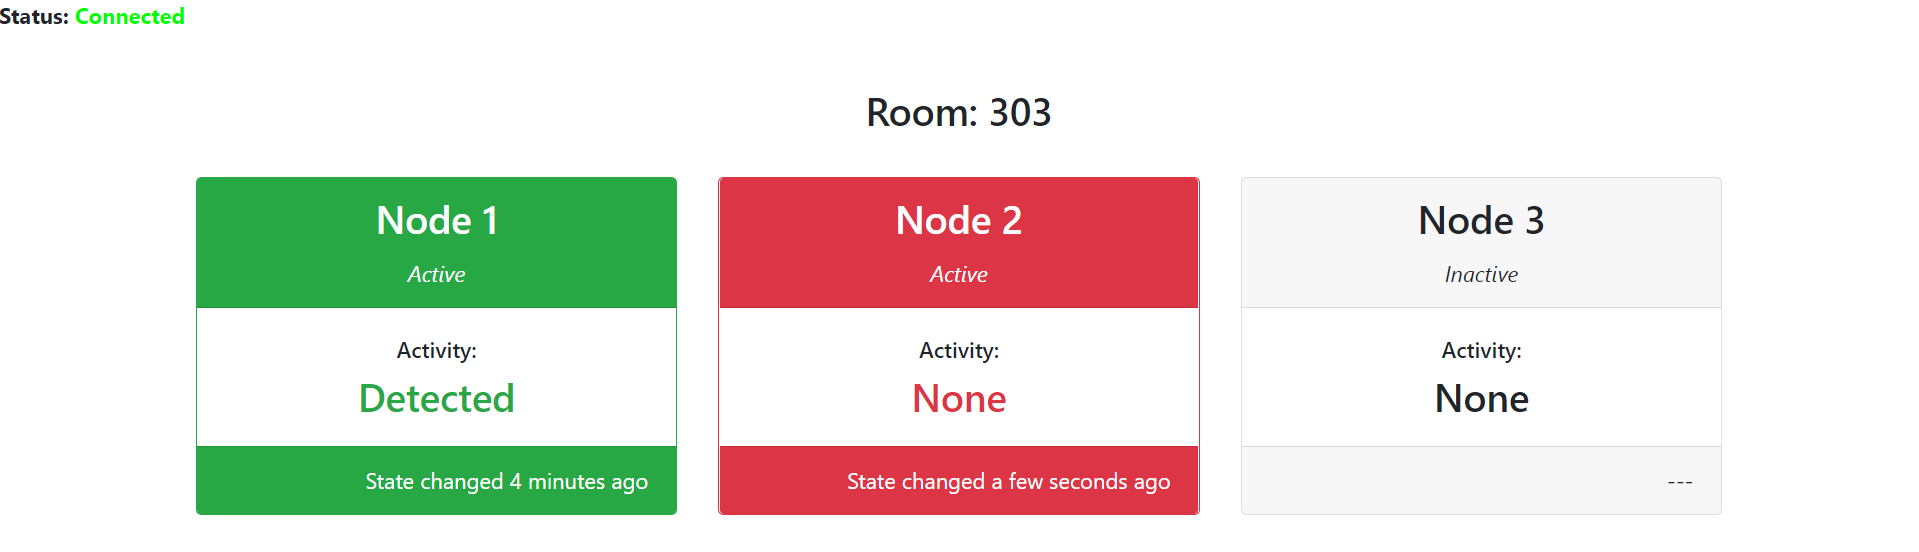
\includegraphics[scale=0.35]{Website1_alternate.PNG}
     Web GUI
\end{center}

Real time occupancy status can be seen on any web browser. The colours indicate state of each node. Green and Red indicate that the node is ON and actively sensing, and their sensor state is represented. The time since the current state has occured is also shown. Greyed out nodes are not active and are either switched OFF or their connection is broken. 

\pagebreak

\begin{center}
	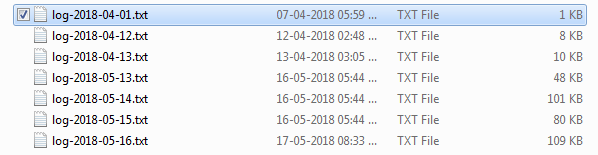
\includegraphics[scale=0.7]{log.png} \\
	Log files generated
	
	\vspace{20pt}
	
	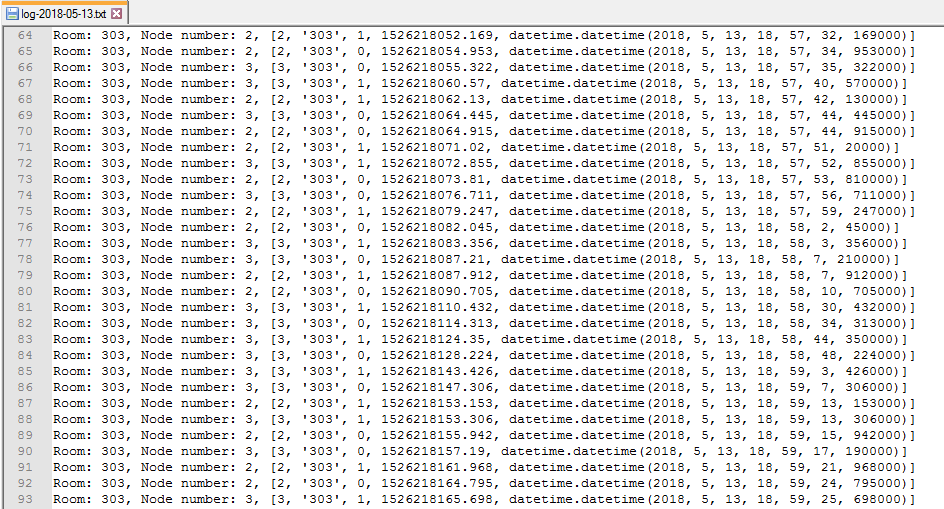
\includegraphics[scale=0.7]{log_sample.png} \\
	A sample log file
\end{center}


The status, location and a precise timestamp of each node gets stored in a log file which can be used to debug or check past sensor states. New log files are generated every day and are organised by date. 





